% WSCG sample document 
%
% based on Gabriel Zachmann's sample
% http://zach.in.tu-clausthal.de/latex/
%
% modified Apr 2012 to match WSCG Word template
%
\documentclass[twoside,twocolumn,10pt]{article}



%%%%%%%%%%%%%%%%%%%%%%%%%%%%%%%%%%%%%%%%%%%%%%%%%%%%%%%%%%%%%%%%%%%%%%%%%%%%%
%                             Packages

\usepackage{wscg}           % includes a number of other packages (e.g., myalgorithm)
\RequirePackage{ifpdf}
\ifpdf
 \RequirePackage[pdftex]{graphicx}
 \RequirePackage[pdftex]{color}
\else
 \RequirePackage[dvips,draft]{graphicx}
 \RequirePackage[dvips]{color}
\fi


\usepackage{nopageno}       % no page numbers at all; uncomment for final version

\usepackage{subfig}
\usepackage{graphicx}
\usepackage[justification=centering]{caption}
\usepackage{amsmath}
\usepackage{algorithm2e}
\usepackage[english]{babel}
%%%%%%%%%%%%%%%%%%%%%%%%%%%%%%%%%%%%%%%%%%%%%%%%%%%%%%%%%%%%%%%%%%%%%%%%%%%%%
%                                Title

\title{Automatic morphology: Application on biological images}

\author{
  \hspace{-0.1\textwidth}
  \parbox{0.2\textwidth}{\centering
    LE Van \\
    Linh\\[1mm]
LaBRI-CNRS 5800\\
ITDLU, Dalat Univ-V
linhlv@dlu.edu.vn/ van-linh.le@labri.fr
}
\hspace{0.02\textwidth}
\parbox{0.2\textwidth}{\centering
BEURTON-AIMAR Marie\\[1mm]
LaBRI-CNRS 5800\\
Bordeaux University\\
33400 Talence-F\\
beurton@labri.fr
}
\hspace{0.02\textwidth}
\parbox{0.25\textwidth}{\centering
KRAHENBUHL \\Adrien\\[1mm]
LaBRI-CNRS 5800\\
Bordeaux University\\
33400 Talence-F\\
adrien.krahenbuhl@labri.fr
}
\hspace{0.02\textwidth}
\parbox{0.18\textwidth}{\centering
PARISEY\\ Nicolas\\[1mm]
IGEPP\\
INRA 1349\\
35653 Le Rheu-F\\
nparisey@rennes.inra.fr
}
}

%%%%%%%%%%%%%%%%%%%%%%%%%%%%%%%%%%%%%%%%%%%%%%%%%%%%%%%%%%%%%%%%%%%%%%%%%%%%%
%                          Hyperref


% no hyperlinks
\usepackage{url}
\urlstyle{tt}

% Donald Arsenau's fix for missing kerning of "//" and ":/"
\makeatletter
\def\Uslash{\mathbin{\mathchar`\/}\@ifnextchar{/}{\kern-.15em}{}}
\g@addto@macro\UrlSpecials{\do \/ {\Uslash}}
\def\Ucolon{\mathbin{\mathchar`:}\@ifnextchar{/}{\kern-.1em}{}}
\g@addto@macro\UrlSpecials{\do : {\Ucolon}}
\makeatother




%%%%%%%%%%%%%%%%%%%%%%%%%%%%%%%%%%%%%%%%%%%%%%%%%%%%%%%%%%%%%%%%%%%%%%%%%%%%%
%                                Document


\begin{document}

\twocolumn[{\csname @twocolumnfalse\endcsname

\maketitle  % full width title


\begin{abstract}
\noindent  Phenotype of species are characterized by several informations like,
  age, sex, morphological measures and environment parameters. Biologists are
  familar to manually getting morphological measures. In the case of
  analysis at the macro level (tissues, small parts of animal \ldots)
  that can be done directly by measuring the element geometry: length,
  width, diameter, angles \ldots. Another way is to take pictures of
  these elements and to run image processing algorithms. From a
  collection of beetle pictures, we have initiated this work to test the
  feasability of automatically positionning landmarks on biological
  images. The set of images contains 293 beetles and for each, an image of the left
  and right mandibles. For each mandible, a set of 16 and 18
  landmarks (resp. left and right) have been manually set. In a previous
  work\cite{leestimating} based on Palaniswamy article \cite{palaniswamy2010automatic} we have shown that
  if we consider the centroid measure of the mandible as the parameter
  to obtain, the probabilistic Hough Transform (PHT) can provide very
  interesting results. But if the goal is to consider more precisely
  the position or the geometry of landmarks area, the results are not
  enough accurate to consider estimated landmarks instead of manual landmarks. In this
  next turn, we have kept the same method to segment and to register
  scene images with a model but we have changed the way to set the
  model landmarks on the scene. This new procedure uses a SIFT
  algorithm as the last operation of our process. SIFT algorithm is
  not applied as usual on the full image but only on areas selected
  by the previous steps. We have compared all
  the obtained results with the previous ones and concluded that this
  new workflow to label the mandible images can be delivered to
  biologist to continue their analysis. This workflow, MAElab is
  available as library function on a github website.
\end{abstract}

\subsection*{Keywords}
Automatic morphology, landmarks identification, image registration.

\vspace*{1.0\baselineskip}
}]



%%%%%%%%%%%%%%%%%%%%%%%%%%%%%%%%%%%%%%%%%%%%%%%%%%%%%%%%%%%%%%%%%%%%%%%%%%%%%


\section{Introduction}

\copyrightspace

In biology, morphology analysis is widely used to keep the changing
information of the organism or detecting the difference information
between the organisms. From the result of morphology analysis, we can
conclude the evolution of an organism family, or we may classify the
organisms. Especially in agriculture, morphology is one of best ways
to learn about the variations of the insect on crops. The morphology
methods may be divided into the groups by the features which are used
by the methods such as shape, structure, color, pattern or size of the
object. In the aim to study the potential links between these
variations and agricultual ecosystems, a set of 291 beetles has been
collected with all the information about the sex, place where they are
found and agricultural practices in each field were recorded. For each
beetle, the morphometric landmarks has been defined on each part (each
insect includes five parts: head, pronotum, body, left and right
mandible) of the insect by the biologies. In this context, we try to
indicate the landmarks on two parts of beetle (left and right mandible
(see figure \ref{figparts})). Morphometric landmarks are points that
can be defined in all speciemns and located precisely. Landmarks are
widely used in many biological studies and they are currently included
into the classification procedures.\\[0.1cm]


\begin{figure}[h]
\centering
\subfloat[Left mandible]{\label{figrbox2}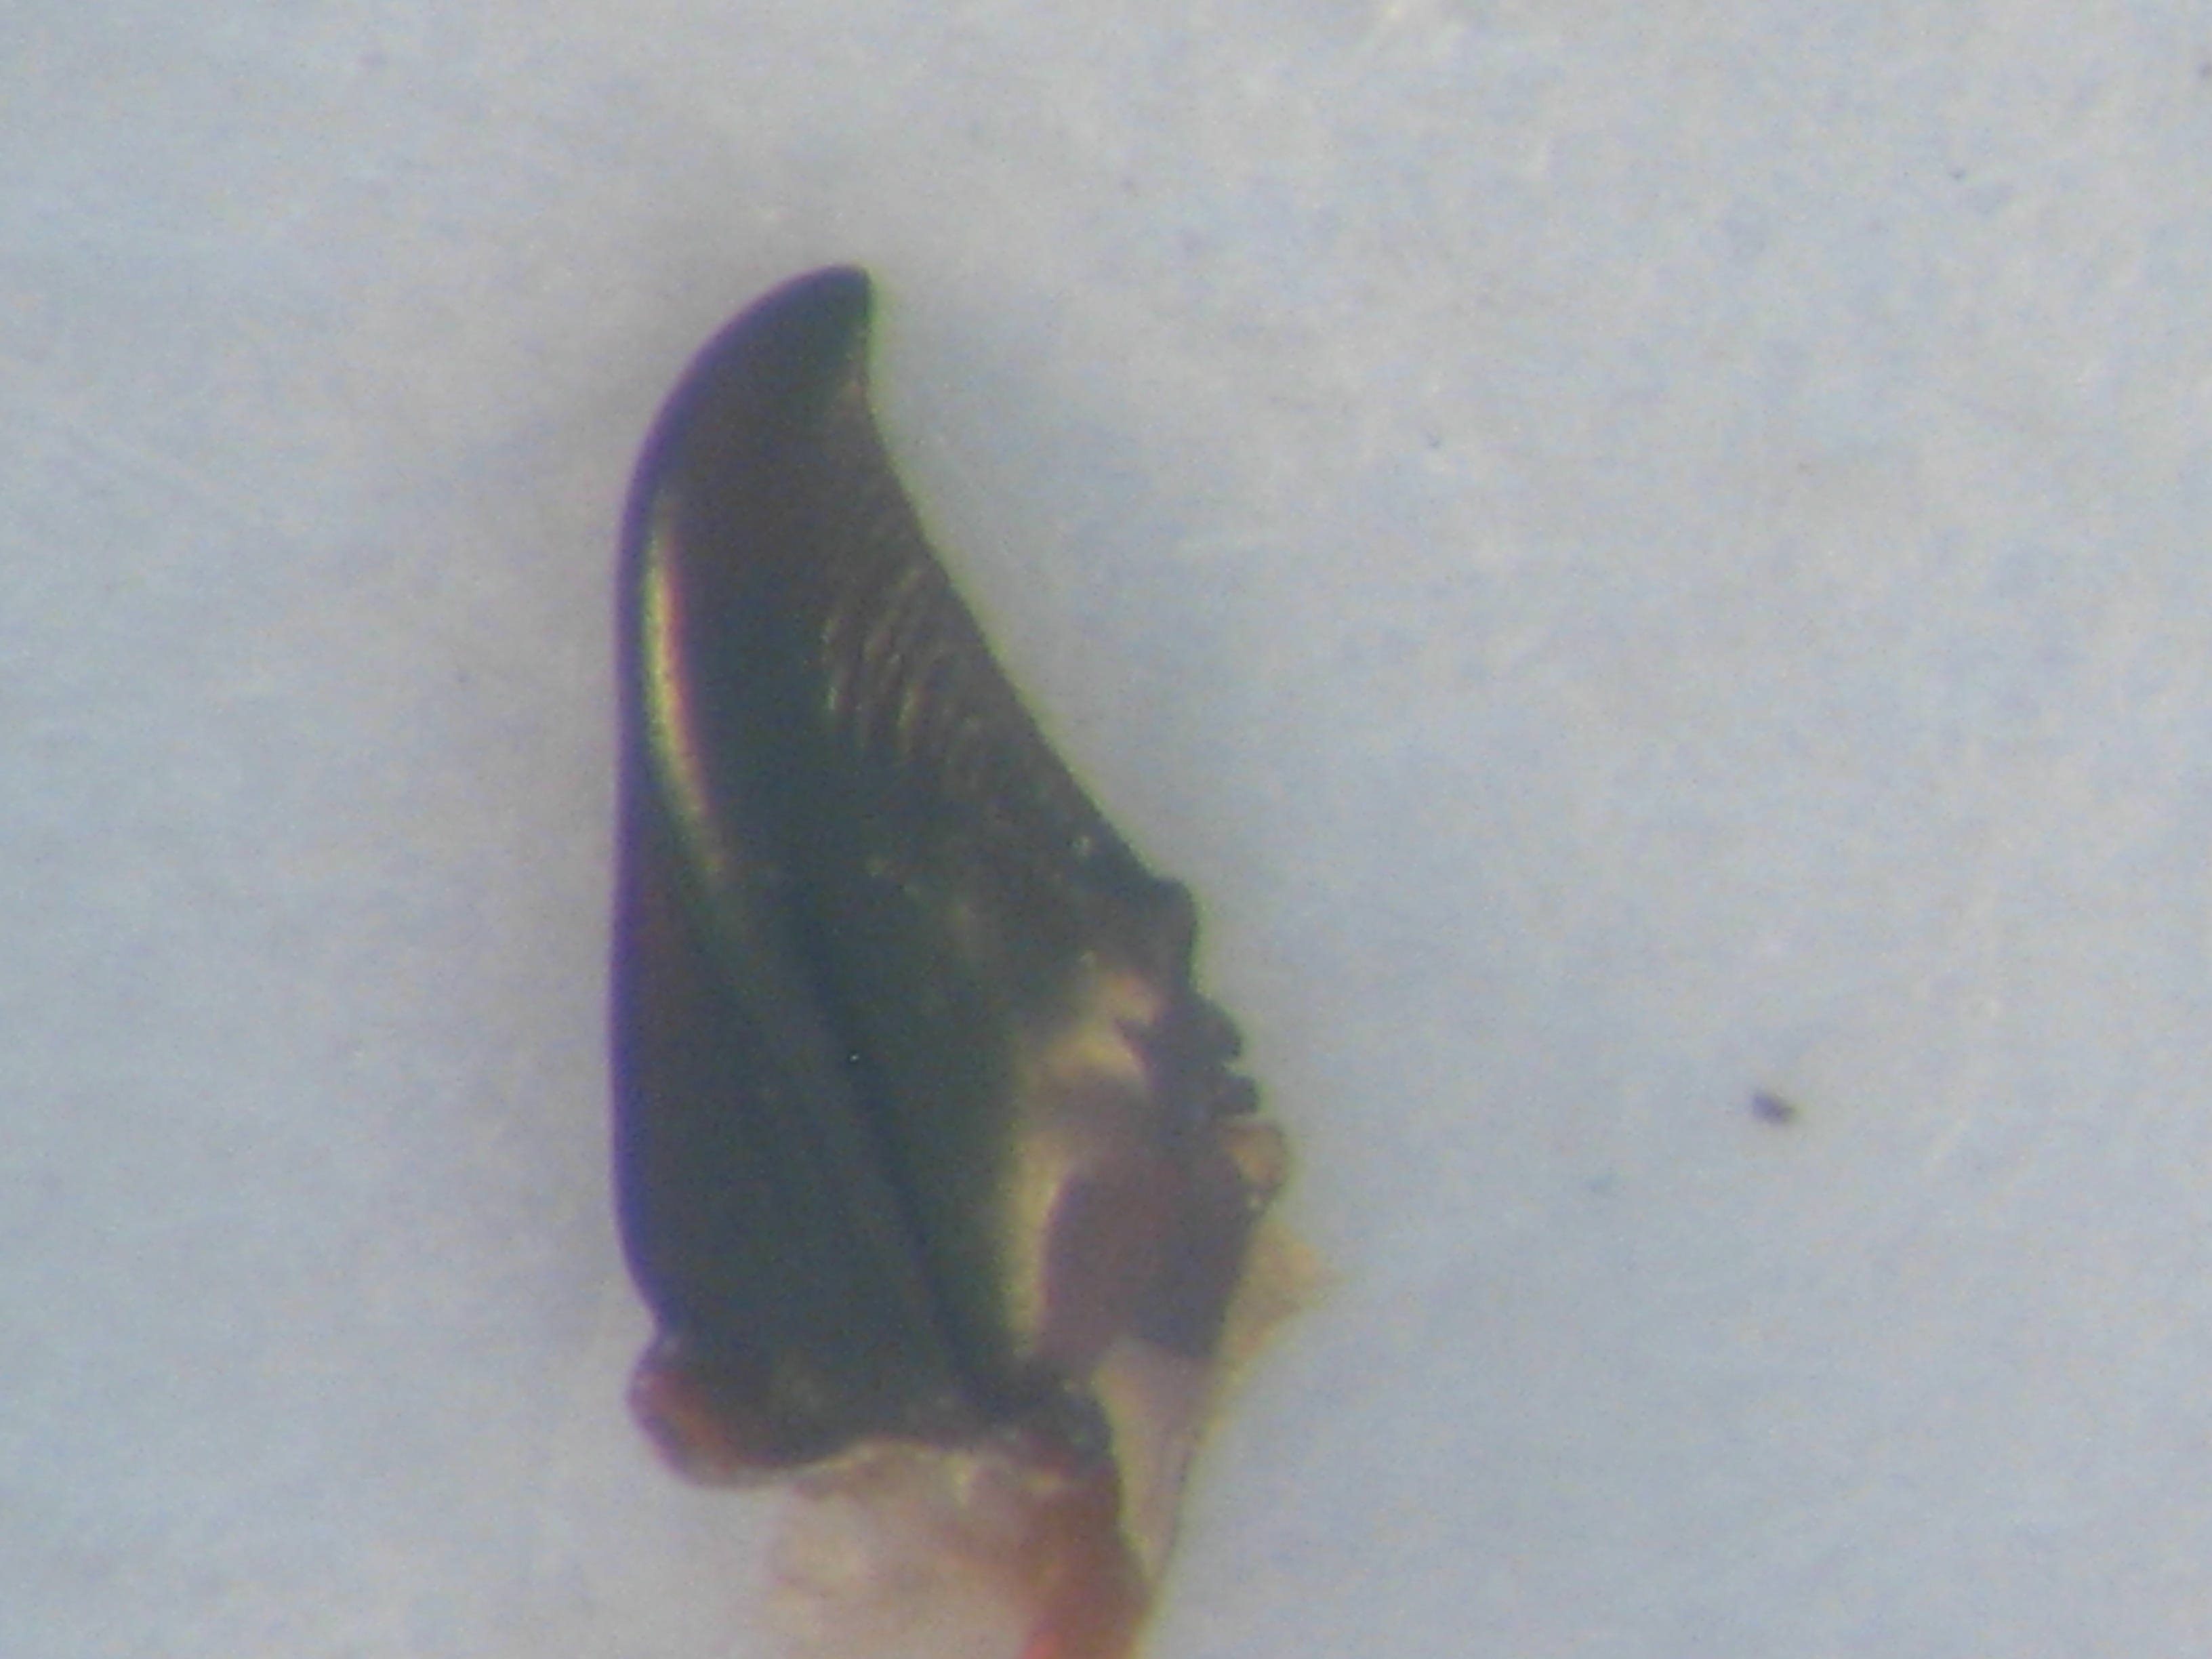
\includegraphics[width=0.22\textwidth]{./images/lm}}~~
\subfloat[Right mandible]{\label{figrbox1}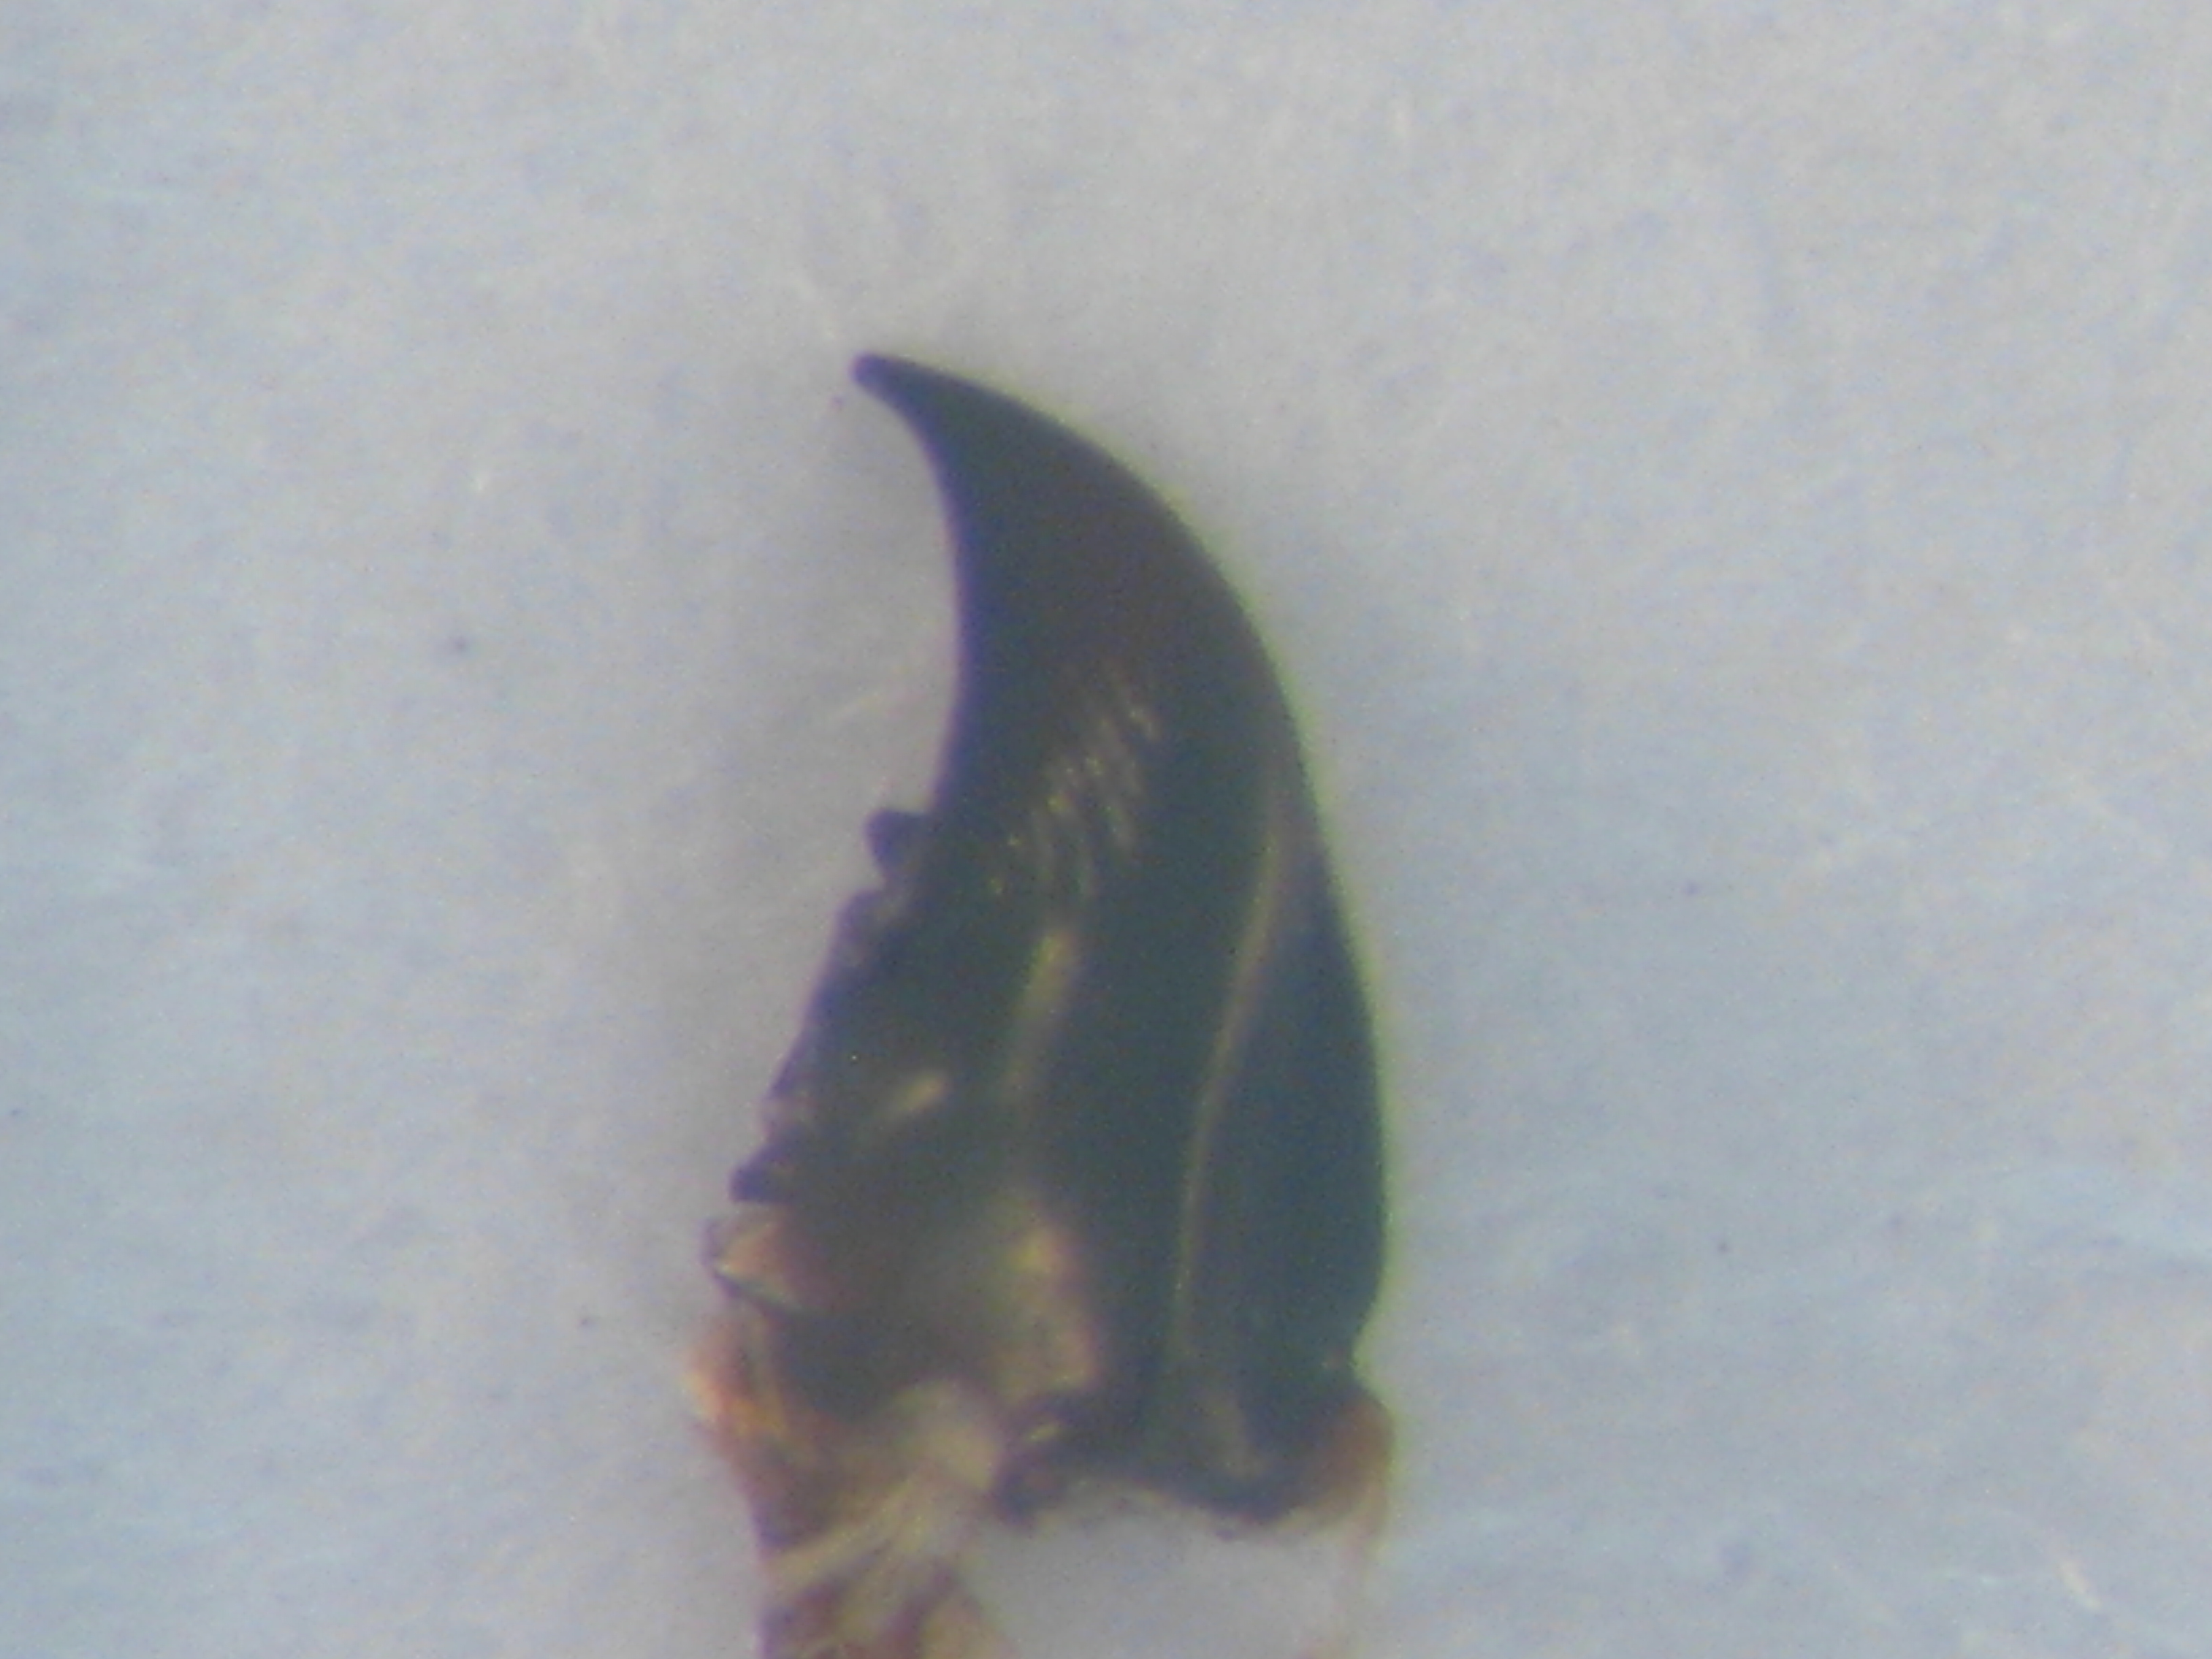
\includegraphics[width=0.22\textwidth]{./images/rm}}
\caption{The mandibles of beetle}
\label{figparts}
\end{figure}~\\[0.1cm]
In this paper, we focus on a method that can automatic identification
of landmarks on 2D images of beetle, specify the mandibles of
beetle. Through whole the article, we use two images to automatic
extraction the landmarks: model image and scene image. The method
mainly includes three stages: firstly, we extract the features of the
object in the image; secondly, principal component analysis iteration is 
used to register two images, the translation and
rotation between two images are also determined; finally, a refinement of
the estimated landmarks is done by SIFT method.\\[0.1cm]

In section 2, the steps of our methods will be presented. All
experiments and evaluation are described in section 3. 

\section{Method}
The problem to solve is to suppress the manual operation of setting
landmarks on each image. To do that we propose a chain of operations,
a workflow, including segmentation step of each image and a registration
with a model image. The model image is more or less chosen randomly, we first
verify by hand that it is not an image of some broken mandibles. The 
figure \ref{fig:method} shows the different steps of the workflow. \\
%%we need to change the drawing a little bit
\begin{figure}[htb]
    \centering
    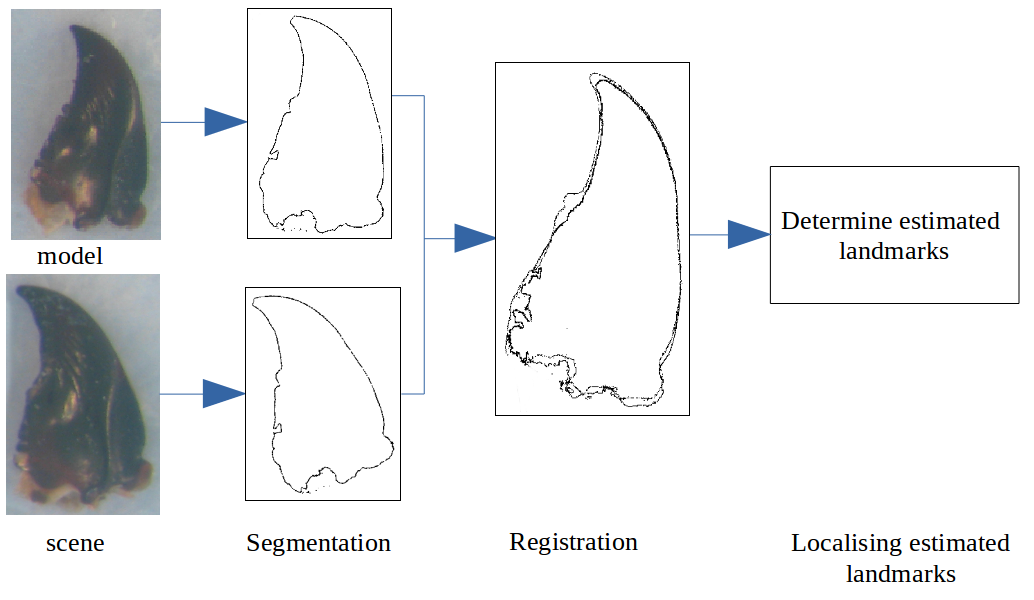
\includegraphics[width=0.5\textwidth]{./images/method}
    \caption{Overview of the proposed method}
    \label{fig:method}
\end{figure}~\\

In this section, we will describe the different algorithms that we have
used. It is worth to note that a protocol to take pictures of each mandible has
been defined. All have been taken in the same conditions, the same
camera with the same resolution.
\subsection{Image segmentation}
Segmentation is often the first task and the bootleneck of image processing
chain. The most well-known algorithms are mainly classified as contours
or regions based segmentation. We have chosen a contours one, the
Canny alogrithm\cite{canny1986computational}, which allows to determine the 
list of edges belonging to the shape of the image.
To use this method, two threshold values have to be set. As it is often mentioned, fixing the right values for these thresholds could be difficult\cite{adaptiveCanny}. The mandatory \textit{threshold
  value} used by Canny algorithm has been determined by analyzing the image
histogram (see \cite{leestimating} for detail). Most often authors define from this threshold, a lower and an upper one. The usual ratio of these two threshold is $T_{lower} = (1/2) * T_{upper}$. In order to consider a larger range of values, we have prefer to set $T_{lower}$ to $1/3$ of $T_{upper}$. For optimisation purpose of the computing time, 
during the computing of Canny algorithm the gradient direction of each pixel which belongs to the
curves is kept for the next steps of the method.\\
\begin{figure}[h]
\centering
\subfloat[Segmentation result after applying Canny
  algorithm]{\label{canny1}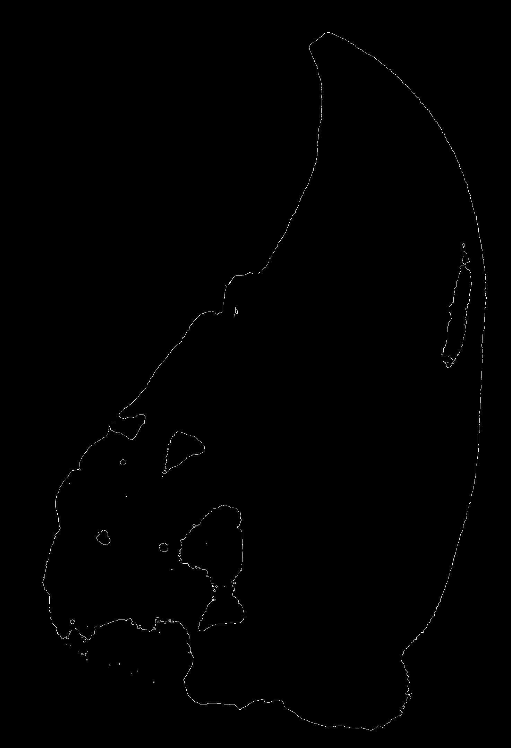
\includegraphics[width=0.2\textwidth]{./images/canny1}}~~ 
\subfloat[Segmentation result after applying Canny algorithm and
  post-process]{\label{canny2}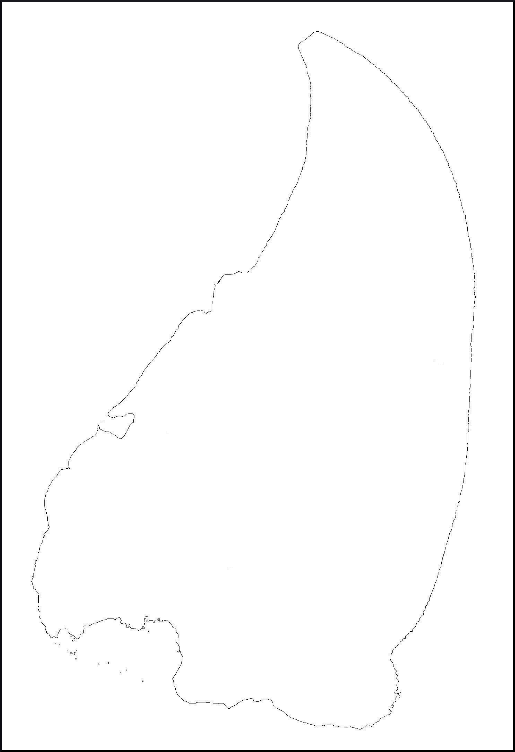
\includegraphics[width=0.2\textwidth]{./images/canny2}} 
\caption{The segmentation results of the image}
\label{canny}
\end{figure}~\\
To achieve the segmentaion step, the obtained contours are post-processed to remove unnecessary
ones. As it is shown in figure \ref{canny}, the final result of Canny generates some contours which do not belong to the shape of the mandible. With a simple algorithm, we browse the image and suppress the edges inside the main shape.
\subsection{Image registration}
As we have mentioned, all images have been captured following the same protocol and at the same scale. But it remains differences in size between the mandibles (cause of size of the beetles), or orientation and position because of the mandible position under the camera. The next step concerns registration of model and scene before estimating the landmarks. Principal Component Analysis Iteration (PCAI) is a well-known method to find the rotation and translation parameter values between two images. In our workflow, we have used a classical PCA computing\cite{bsspca}, \cite{shlens2014tutorial}.\\

As input values, we use the lists of points which has been defined by the segmentation step. Firstly, the centroid point and principal axis of each image are defined: the centroid point is the point which has the coordinate equal to the mean coordinate of all boundary points; the principal axis is a connected line from the centroid point to a point in the list of countours points. The second endpoint on curve points are determined as described: For each point in the curve, we assume that it is the second endpoint of the principal axis. Then, the mean of the perpendicular distance from the remaining points to the axis is calculated. When the computing is finished, the principal axis is the line that has the minimum mean perpendicular distance to all points of the contours. The translation is indicated by the coordinate difference between the centroid points of the scene and the model. The rotation angle is the angle between the principal axes of these two images. \textbf{As well as, the rotation direction is determined by checking on each direction}. Then, the scene is moved to matching with the position of the model. However,
in some case, the translation and rotation between two images are
not enough right because the result of the segmentation may be not perfect. To improve registration, we have enhanced the PCA by an iteration state (PCAI). We have considered some specificity of our images and observed that the tip part of the mandible is less noisy than the base. So, we sort the points according to their y-value. We build a subset of points which contains half part of points, these ones which belong to the upper part of the image. PCA is again completed for this subset to refine the rotation and translation values. This operation is iterated until the new computing angle is less than 1.5 degree (see figure \ref{fig:pcai}).
\begin{figure}[htb]
    \centering
    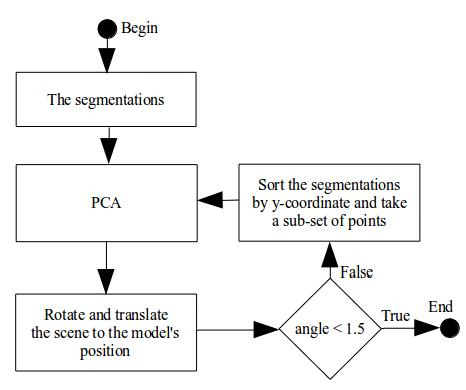
\includegraphics[width=0.4\textwidth]{./images/pcadiagram}
    \caption{The flows in PCAI}
    \label{fig:pcai}
\end{figure}~\\
Figure \ref{fig:box} shows an example obtained results from the different steps of PCAI. In this figure, the red contours is the model segmentation, the black contours is the scene segmentation after one iteration, and the blue contours is the last result after finished PCAI .\\

\begin{figure}[htb]
    \centering
    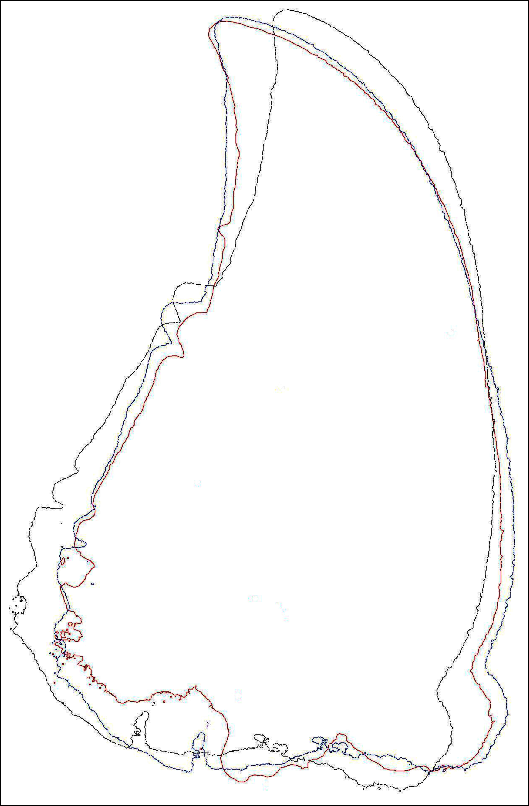
\includegraphics[width=0.25\textwidth]{./images/imreg}
    \caption{Differnent registration steps between two images}
    \label{fig:box}
\end{figure}
\subsection{Fixing the estimated landmarks}
The last task in the workflows concerns how to estimate landmarks of the scene from the manual ones of the model. This has to be done by using SIFT\cite{lowe2004distinctive} method but as usually we not consider all points of the image but only the area around the landmarks. Firstly, the region around each manual landmark in the model is created and its corresponding position in the scene image is defined. Then, the SIFT descriptor is computed\textbf{xxx}.

The comparesion between the SIFT descriptors is done by using $L2$ distance which is given by the equation (1).
\begin{equation}
\label{eq:cross-correlation}
	L(x,y) = \sum\limits_{x_i,y_i}\sqrt{(x_i-y_i)^2}
\end{equation}
Where $x, y $ are the descriptors; $x_i, y_i $ are the corresponding location in the descriptors.\\

The figure \ref{fig:Illustrate} is the illustration of this process. For each manual landmark on the model and corresponding estimated landmark on the scene, the patches \textit{$P_m, P_s$} are created(size of $P_m$ $<$ size of $P_s$). For each pixel in the patch \textit{$P_s$}, a sub-patch \textit{$T^{'}_s$} is extracted with the same size of \textit{$P_m$}. Then, their descriptor and measure distance are calculated (between \textit{$P_m$} and \textit{$T^{'}_s$}). This process is finished when all the pixels on the patch \textit{$P_s$} are considered. The coordinates of estimated landmark is the location in \textit{$P_s$} that has the smallest measure distance value with \textit{$P_m$}. Finally, the coordinates of the estimated landmarks is set to the original location of the scene image by applying the reverse operation of rotation and translation.
\begin{figure}[htb]
    \centering
    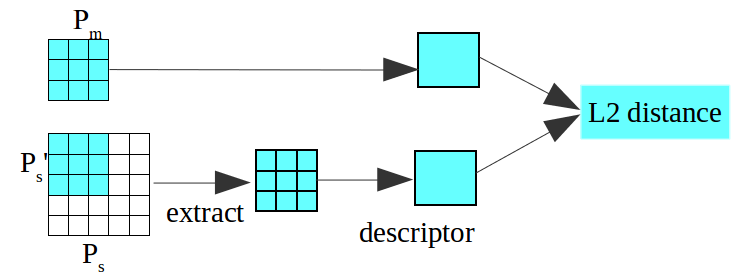
\includegraphics[width=0.48\textwidth]{./images/illustration_SIFT}
    \caption{Illustrate the steps of descriptors comparison.}
    \label{fig:Illustrate}
\end{figure}

During the descriptor creation (\textit{$I$} and \textit{$T^{'}$}), the orientation and gradient magnitude are calculated for each their pixel by the equation:
\begin{equation}
\label{eq:sift}
\resizebox{.41 \textwidth}{!} 
{$
\begin{aligned}
	m(x,y) = \sqrt{(L(x+1,y) - L(x-1,y))^2 + (L(x,y+1) - L(x,y-1))^2} \\
	\theta(x,y) = tan^{-1}((L(x,y+1) - L(x,y-1))/(L(x+1,y) - L(x-1,y)))
	\end{aligned}
$}
\end{equation}
Where:
\begin{itemize}
	\item $m(x,y)$ is the gradient magnitude of the pixel at position (x,y)
	\item $\theta(x,y)$ is the orientation of the pixel at position (x,y)
	\item $L(x,y)$ is the value at position (x,y) in the image
\end{itemize}
Then, the descriptor is created for the patch. This is a histogram with eight direction for orientation, with the length of each bin is sum of the gradient magnitude of the pixels that corresponding  with the orientation. The descriptor is formed from a vector containing the value of all the bins in the histogram. Finally, the vector feature is modified to reduce the effects of illumination change by normalization.

\begin{figure}[htb]
    \centering
    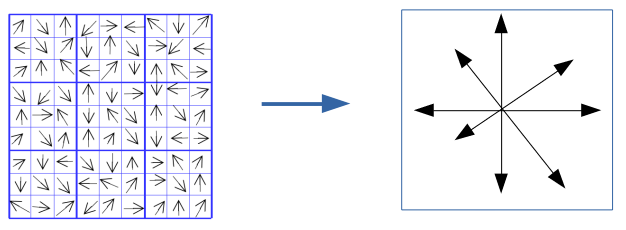
\includegraphics[width=0.4\textwidth]{./images/keypoint_descriptor}
    \caption{A landmarks descriptor is created by computing the orientation and gradient magnitude}
    \label{fig:kpdescriptor}
\end{figure}

In the example at figure \ref{fig:kpdescriptor}, a patch with the size 16x16 is created around the landmark. For each pixel in the region, the orientation and gradient magnitude are calculated (the orientation and length of the arrows). Then, the patch is divided into 4 sub-blocks 4x4. The descriptor of each sub-block is determined by using 8-orientation histogram and the length of each arrow corresponding to the sum of the gradient magnitudes near that direction within the region.\\

\section{Experiments and result}
All the steps in our method are implemented in MAELab\footnote{MAELab
  is a free software in C++. It can be directly obtained by request
  the authors.}. Two sets of beetle have been analyzed, right and left
mandibles. After verifying the quality of the image, it remains 290
usable images for right mandible and 286 images for the left mandible. The
removed images include the images that do not contain the mandible or
the borken mandibles. Then, each dataset is divided into two sub-sets followed the size of the mandible. For each subset, an image is chosen as the model of the experiment process. In all valid images, a set of 18 manual landmarks of right mandible (16 landmarks for left mandible) are indicated by biologists. Along with choosing the centroid size to measure the mandible. This size is obtained by sum of all square distance from each landmarks to the
centroid point (see \cite{web2010}).\\

At the end of PCAI, a hypothesis is made to estimated the scale between the images. For each image, the bounding boxes are indicated by the coordinates of the points on the curve. The scale of x and y-direction are determined by the ratio between the corresponding sides of the bounding boxes. Then, the scene curve is scaled to fit the model curve. 
\begin{figure}[h]
\centering
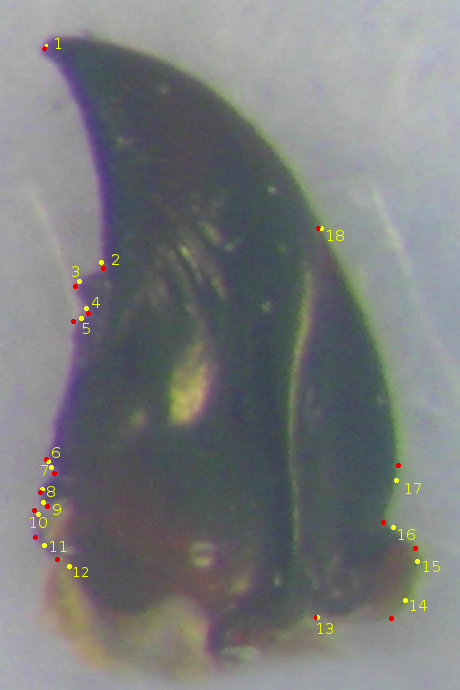
\includegraphics[width=0.4\textwidth]{./images/md_rs}
\caption{The automatic landmarks on right mandible}
\label{figresult}
\end{figure}~\\
Figure \ref{figresult} shows a complete result on one right mandible with the manual landmarks (red points) and estimated landmarks (yellow points). As we can see in the image, almost the estimated landmarks are quite near with the manual landmarks. This shows that our method is worked well for indicating the landmarks on the mandibles.\\

In next experiment, we want focus soon on two kinds of evaluation: centroid size of the image and the accuracy position of each landmark.
\begin{figure}[htb]
    \centering
    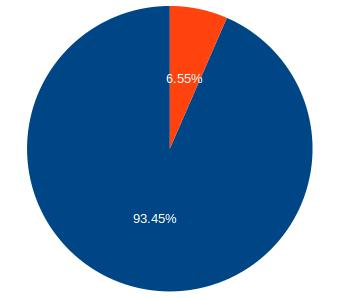
\includegraphics[width=0.3\textwidth]{./images/mdresult}
    \caption{The percentage of correct proportions on right mandibles }
    \label{figmdresult}
\end{figure}~\\
\begin{figure}[htb]
    \centering
    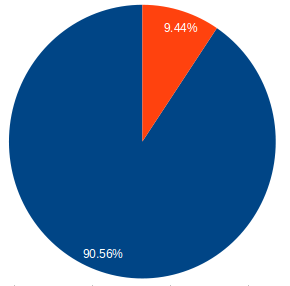
\includegraphics[width=0.3\textwidth]{./images/mgresult}
    \caption{The percentage of correct proportions on left mandibles }
    \label{figmgresult}
\end{figure}~\\
Firstly, our evaluation is done on comparing the centroid size of the estimated landmarks and manual landmarks. The experiment is done by choosing an arbitrary 
image in the dataset as the model. The automatic landmarks are estimated on remaining images with the method that we have described. Then, the centroid size of each image is calculated and evaluated. We can see in figure
\ref{figmdresult} and figure \ref{figmgresult} for all images, the
correct proportions of centroid size which based on the estimated landmarks are 93,45\% for the right
mandible and 90,21\% for the left mandible with the standard deviation\cite{bland1996statistics}. And the results in figure \ref{figmdresult} and \ref{figmgresult} were a vindication of the propriety of the method.\\

Besides using the centroid size to evaluate the method. We are also
interested in the accuracy on the position of the estimated landmarks. In this experiment
way, we calculate the distance between each manual landmark and
corresponding automatic landmark. Through, we want to examine replacing the manual landmarks by corresponding estimated landmarks.
\begin{figure}[htb]
    \centering
    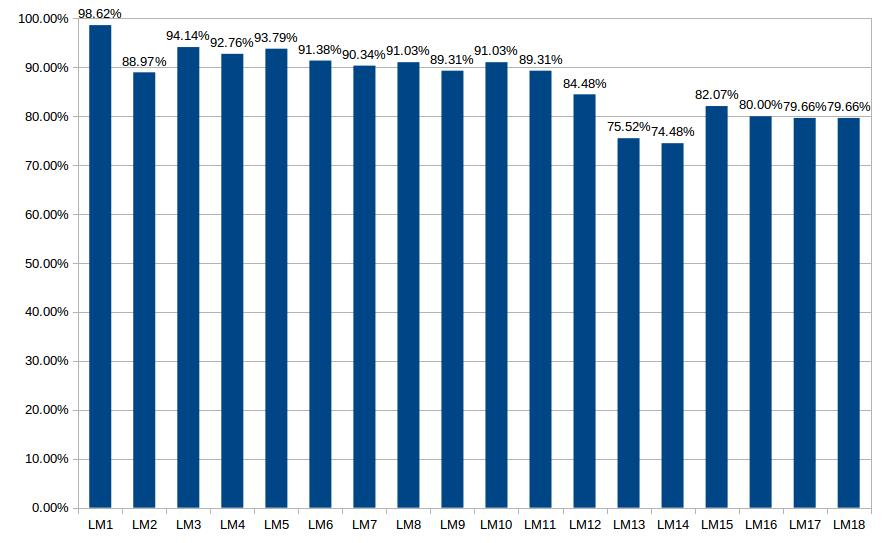
\includegraphics[width=0.5\textwidth]{./images/md_chartlms}
    \caption{The correct proportions on each landmark of right mandibles }
    \label{figmdresultlm}
\end{figure}~\\
\begin{figure}[htb]
    \centering
    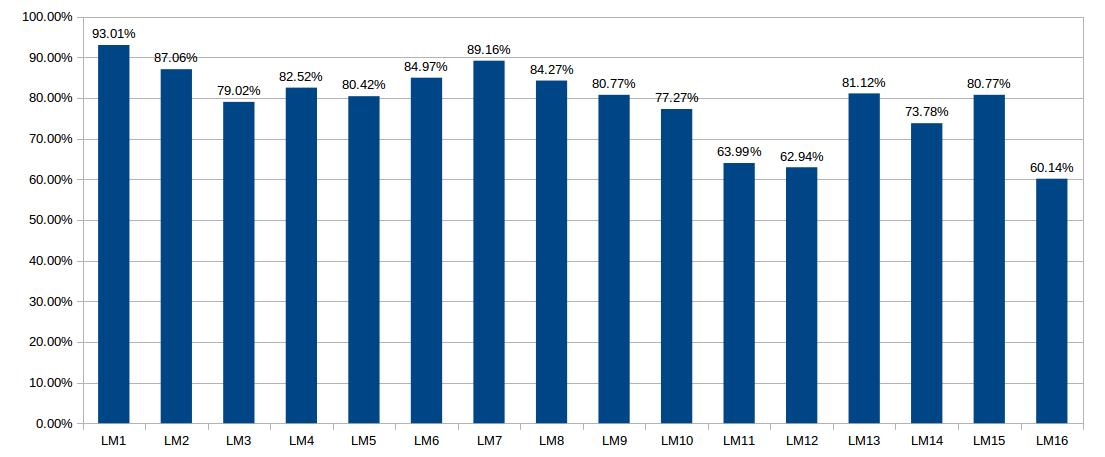
\includegraphics[width=0.5\textwidth]{./images/mg_chartlms}
    \caption{The correct proportions on each landmark of left mandibles }
    \label{figmgresultlm}
\end{figure}~\\
Figure \ref{figmdresultlm} and \ref{figmgresultlm} show the correct proportion on each landmark of mandible. The blue column is presented for the success rate. The orange column is expressed as the incorrect rate. With 18 landmarks of right mandible, the position of the first estimated landmarks is reasonably accurate with 98.62\%, the lowest proportion is 74,48\% for fourteenth landmark. The remaining landmarks are also indicated with a high proportion (with the accuracy proportion greater than 75\%). For left mandible, the highest and lowest success rate are 93,01\% for the first landmark and 60,14\% for the sixteenth landmark. The statistic is done on each automatic landmarks of all the images with a standard deviation\cite{bland1996statistics}. \\

In both of experiments, the success rate on right mandible is always greater than left mandible. So, when we reconsider the datasets, the images in left mandible are having more type of size than on the right mandible (scale problem). This explains why the success rate on right mandible is always higher than left mandible.\\

From two experiment ways, we can see that the method is success in
indicating all landmarks for each image; and the location of the
landmarks is considered near with the manual landmarks in some
aspect. In a different side, when comparing with our previous study (see in
\cite{leestimating}). This method has more exactly about the position of
automatic landmarks as well as the advantages for the implementation
process. The memory to detecting the landmarks, along with the times
to execute the process are decreased dramatically.

\section{Conclusion}
Morphometric analysis is a powerful tool in biology in classification
the species. Automatic identification the characteristics biology of
the organism is a difficult problem. In the content of this paper, we
have begun to design a method to segment the beetle mandibles and to
indicate automatically landmarks which have been determined by
biologists. Each mandible is segmented by applying the Canny
algorithm. Using PCAI to align the images and estimate the
landmarks. Finally, a descriptor distance will be applied to refine the
location of the estimated landmarks. The first version of this method
has been implemented. From now, the next stage of our method is to add
the features to have the position of landmarks more precisely, i.e diagnose on the scale of the image.


\bibliographystyle{plain}
\bibliography{references}

\end{document}

%-------------------------------------------------------------------------
% example of algorithm typesetting
% to allow this, uncomment line 
% \RequirePackage[noend]{myalgorithm}
% in the wscg.sty file
% and download that package from Gabriel Zachmann's page http://zach.in.tu-clausthal.de/latex/
%
%
%\begin{algorithm}
%\hrule
%  \centering
%\begin{algorithmic}
%    \STMT $d_{l,r} = f_B(P_1), f_B(P_n)$
%    \WHILE{ $|d_l| > \epsilon $ and $|d_r| > \epsilon $ and $l<r$}
%        \STMT $d_x = f_B(P_x)$
%        \IF{ $d_x < 0$ }
%            \STMT $l, r = x, r$
%        \ELSE
%            \STMT $l, r = l, x$
%        \ENDIF
%    \ENDWHILE
%\end{algorithmic}
%\hrule
%\caption{Example of some pseudo-code}
%\label{fg:code}
%\end{algorithm}

%-------------------------------------------------------------------------

\begin{thebibliography}{99}
\label{references}
\bibitem[1]{canny} Canny, John. "A computational approach to edge detection." IEEE Transactions on pattern analysis and machine intelligence 6 (1986): 679-698.
\bibitem[2]{Ballard} Ballard, Dana H. "Generalizing the Hough transform to detect arbitrary shapes." Pattern recognition 13.2 (1981): 111-122.
\bibitem[3]{Webster} Webster, M. A. R. K., and H. DAVID Sheets. "A practical introduction to landmark-based geometric morphometrics." Quantitative Methods in Paleobiology 16 (2010): 168-188.
\bibitem[4]{est} Le Van, L., et al. "Estimating landmarks on 2D images of beetle mandibles."
\bibitem[5]{pca} Shlens, Jonathon. "A tutorial on principal component analysis." arXiv preprint arXiv:1404.1100 (2014).
\bibitem[6]{sift} Lowe, David G. "Distinctive image features from scale-invariant keypoints." International journal of computer vision 60.2 (2004): 91-110.
\bibitem[7]{palaniswamy} Palaniswamy, Sasirekha, Neil A. Thacker, and Christian Peter Klingenberg. "Automatic identification of landmarks in digital images." IET Computer Vision 4.4 (2010): 247-260.
\end{thebibliography}

%{\bfseries
%Last page should be fully used by text, figures etc. Do not leave empty space, please. 

%Do not lock the PDF -- additional text and info will be inserted, i.e. ISSN/ISBN etc. 
%}

